\subsection{Ручные методы}

Ручные методы обеспечения качества программного обеспечения представляют собой с одной стороны, самые простые с точки зрения применения, но, с другой стороны, самые ненадежные способы удостовериться в том, что ПО выполняет возложенные на него задачи. Под ручными методами мы будем понимать все методы, которые не предполагают или не поддаются какой-либо автоматизации.

К таким методам можно отнести, например, код-ревью или тестирование программного обеспечения.

Код-ревью или просмотр кода -- это инженерная практика, заключающаяся в том, что код программы просматривается одним или несколькими разработчиками с целью обнаружения дефектов или же совершенствования навыков разработчика.

Исторически, первым упоминанием код-ревью можно считать работу Майкла Фагана(англ. Michael Fagan) \cite{fagan1999design}, в которой он предлагает методологию нахождения дефектов в программном коде путем его инспекций.

По Фагану, процесс инспекции представляет собой сравнение выхода каждой операции с некоторым выходным критерием. Кроме выходных критериев Фаган вводит входные критерии -- критерии, которым должна удовлетворять операция перед ее началом.

Более подробно, процесс инспекции состоит из следующих операций:

\begin{enumerate}
  \item Планирование(\textit{Planning}). Включает в себя подготовку материалов(кода), места для встречи и встречи участников.
  \item Обзор(\textit{Overview}). Включает ознакомление участников процесса с материалами и назначение ролей.
  \item Подготовка(\textit{Preparation}). Включает непосредственный обзор участниками материалов с целью выяснения возможных дефектов.
  \item Обсуждение(\textit{Inspection meeting}). Включает непосредственное нахождение дефектов.
  \item Исправления(\textit{Rework}). Найденные дефекты исправляются их авторами
  \item Заключение(\textit{Follow-up}). Финальный этап, на котором участники удостоверяются, что все найденные дефекты исправлены и процесс исправлений не породил новых.
\end{enumerate}

\begin{figure}[H]
  \centering
  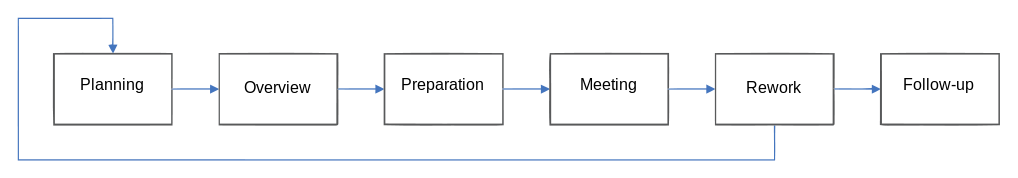
\includegraphics[width=\textwidth]{img/fagan.png}
  \caption{Процесс инспекции кода по Фагану}
\end{figure}

Помимо инспекции кода существует еще и большое количество видов тестирования программного обеспечения. Как-то:

\begin{enumerate}
  \item Функциональное тестирование
  \item Системное тестирование
  \item Тестирование производительности
  \item Регрессионное тестирование
  \item Модульное тестирование
  \item и т.д.
\end{enumerate}

Нас больше интересует так называемое ручное тестирование в ходе которого инженер использует продукт, моделируя действия конечного пользователя. Предыдущие виды тестирования так или иначе используют программные средства для запуска или анализа кода, поэтому его можно отнести скорее к динамическим методам.

Основная идея ручного тестирования заключается в том, что бы посмотреть на систему с точки зрения пользователя и увидеть недостатки в качестве ПО, которые не сразу заметны в ходе разработки. Этот вид тестирования довольно неплохо работает, например, для пользовательских интерфейсов.

Более или менее очевидно, что ручные методы плохо справляются со сложными системами, либо же требуют слишком много времени и усилий. Поэтому далее мы рассмотрим две группы методов, которые используют программные средства и являются более выразительными в том смысле, что позволяют проверить более строгие инварианты в программном коде.
